\subsection{连接同态与正合序列}

设 M 为一个 A-模。回顾：对于每个 A-模 N，我们在前一小节中定义了 k-模的同构

\[
\varphi_ {\mathbf {M}} (\mathbf {N}): \mathrm{H} (\operatorname{Homgr} _ {\mathbf {A}} (\mathrm{L} (\mathbf {M}), \mathbf {N})) \rightarrow \operatorname{Ext} _ {\mathbf {A}} (\mathbf {M}, \mathbf {N}).
\]

设

\[
0 \to \mathbf {N} ^ {\prime} \xrightarrow {u} \mathbf {N} \xrightarrow {v} \mathbf {N} ^ {\prime \prime} \to 0\tag{$(\mathcal{E})$}
\]

一个 A-模的正合序列；k-复形序列

\[
\begin{array}{r l} \left(\mathbf {M} ^ {\mathcal {E}}\right) & 0 \longrightarrow \operatorname{Homgr} _ {\mathbf {A}} (\mathrm{L} (\mathrm{M}), \mathrm{N} ^ {\prime}) \xrightarrow {\operatorname{Homgr} (1 , u)} \operatorname{Homgr} _ {\mathbf {A}} (\mathrm{L} (\mathrm{M}), \mathrm{N}) \\ & \xrightarrow {\operatorname{Homgr} (1 , v)} \operatorname{Homgr} _ {\mathbf {A}} (\mathrm{L} (\mathrm{M}), \mathrm{N} ^ {\prime \prime}) \longrightarrow 0 \end{array}
\]

于是是正合的（X，第 83 页，命题 2，a）），即

\[
\partial_ {(\mathbf {M} ^ {\mathcal {E}})}: \mathrm{H} (\operatorname{Homgr} _ {\mathbf {A}} (\mathrm{L} (\mathbf {M}), \mathrm{N} ^ {\prime \prime})) \rightarrow \mathrm{H} (\operatorname{Homgr} _ {\mathbf {A}} (\mathrm{L} (\mathbf {M}), \mathrm{N} ^ {\prime}))
\]

相应的连接同态（X，第 29 页）。

定义2.——相对于模 M 与正合序列（\(\mathcal{E}\)）的扩张模的连接同态称为复合同态

\[
\delta (\mathbf {M}, \mathcal {E}) = \varphi_ {\mathbf {M}} (\mathbf {N} ^ {\prime}) \circ \partial_ {(\mathbf {M} ^ {\mathcal {E}})} \circ \varphi_ {\mathbf {M}} (\mathbf {N} ^ {\prime \prime}) ^ {- 1}: \operatorname{Ext} _ {\mathbf {A}} (\mathbf {M}, \mathbf {N} ^ {\prime \prime}) \rightarrow \operatorname{Ext} _ {\mathbf {A}} (\mathbf {M}, \mathbf {N} ^ {\prime}).
\]

这是一个 \(k\) -分次同态，其次数递增 1，其齐次分量记为 \(\delta^n (\mathbf{M},\mathcal{E})\colon \mathrm{Ext}_{\mathbf{A}}^{n}(\mathbf{M},\mathbf{N}^{\prime \prime})\to \mathrm{Ext}_{\mathbf{A}}^{n + 1}(\mathbf{M},\mathbf{N}^{\prime})\) .

定理1. --- k-模同态的右无界序列

\[
\begin{array}{r l} 0 & \xrightarrow {\quad} \mathrm{Hom} _ {A} (M, N ^ {\prime}) \xrightarrow {\mathrm{Hom} (1 , u)} \mathrm{Hom} _ {A} (M, N) \xrightarrow {\mathrm{Hom} (1 , v)} \mathrm{Hom} _ {A} (M, N ^ {\prime \prime}) \\ & \xrightarrow {\delta (M , \mathcal {E})} \mathrm{Ext} _ {A} ^ {1} (M, N ^ {\prime}) \to \dots \xrightarrow {\delta^ {n - 1} (M , \mathcal {E})} \mathrm{Ext} _ {A} ^ {n} (M, N ^ {\prime}) \xrightarrow {\mathrm{Ext} ^ {n} (1 , u)} \mathrm{Ext} _ {A} ^ {n} (M, N) \\ & \xrightarrow {\mathrm{Ext} ^ {n} (1 , v)} \mathrm{Ext} _ {A} ^ {n} (M, N ^ {\prime \prime}) \xrightarrow {\delta^ {n} (M , \mathcal {E})} \mathrm{Ext} _ {A} ^ {n + 1} (M, N ^ {\prime}) \to \dots \end{array}
\]

是正合的。

的确，考虑 X 第 91 页上的图表。

由 X 第 88 页的注记 3 及定义 2，它是交换的；此外，底行是正合的（X，第 30 页，定理 1），且竖直箭头是双射的（X，第 88 页，命题 5）。

推论. —— 若 Ext \(_{A}^{1}\) (M, N') = 0，该序列

\[
0 \longrightarrow \operatorname{Hom} _ {\mathbf {A}} (\mathrm{M}, \mathrm{N} ^ {\prime}) \xrightarrow {\operatorname{Hom} (1 , u)} \operatorname{Hom} _ {\mathbf {A}} (\mathrm{M}, \mathrm{N}) \xrightarrow {\operatorname{Hom} (1 , v)} \operatorname{Hom} _ {\mathbf {A}} (\mathrm{M}, \mathrm{N} ^ {\prime \prime}) \longrightarrow 0
\]

是正合的。

命题8。——设 \(f: \mathbf{M}_{1} \to \mathbf{M}\) 是 A-模的同态，且

\[
0 \longrightarrow \mathbf {N} ^ {\prime} \stackrel {u} {\longrightarrow} \mathbf {N} \stackrel {v} {\longrightarrow} \mathbf {N} ^ {\prime \prime} \longrightarrow 0\tag{$(\mathcal{E})$}
\]

\[
g ^ {\prime} \Big \downarrow \qquad \qquad g \Big \downarrow \qquad \qquad g ^ {\prime \prime} \Big \downarrow
\]

\[
0 \longrightarrow \mathrm{N} _ {1} ^ {\prime} \stackrel {u _ {1}} {\longrightarrow} \mathrm{N} _ {1} \stackrel {v _ {1}} {\longrightarrow} \mathrm{N} _ {1} ^ {\prime \prime} \longrightarrow 0\tag{$(\mathcal{E}_1)$}
\]

\pandocbounded{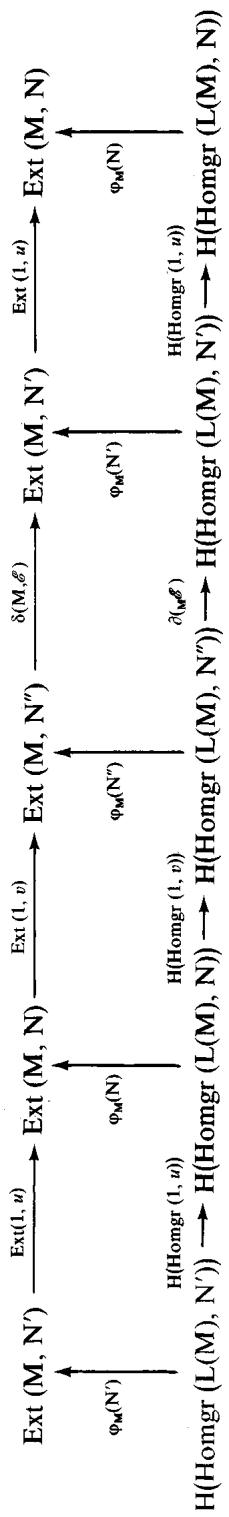
\includegraphics[keepaspectratio]{images/part001_97747f10.jpg}}

是 A-模的具有正合行的交换图。则 k-模的图

\[
\begin{array}{c} \operatorname{Ext} _ {\mathbf {A}} (\mathbf {M}, \mathbf {N} ^ {\prime \prime}) \xrightarrow {\delta (\mathbf {M} , \mathcal {E})} \operatorname{Ext} _ {\mathbf {A}} (\mathbf {M}, \mathbf {N} ^ {\prime}) \\ \operatorname{Ext} (f, g ^ {\prime \prime}) \Big | _ {\downarrow} \qquad \qquad \qquad \qquad \qquad \qquad \qquad \qquad \qquad \qquad \qquad \qquad \qquad \qquad \qquad \qquad \qquad \qquad \qquad \qquad \qquad \qquad \qquad \qquad \qquad \qquad \qquad \qquad \qquad \qquad \qquad \qquad \qquad \qquad \\ \operatorname{Ext} _ {\mathbf {A}} (\mathbf {M} _ {1}, \mathbf {N} _ {1} ^ {\prime \prime}) \xrightarrow {\delta (\mathbf {M} , \mathcal {E} _ {1})} \operatorname{Ext} _ {\mathbf {A}} (\mathbf {M} _ {1}, \mathbf {N} _ {1} ^ {\prime}) \end{array}
\]

是交换的。

这由 X，第 31 页，命题 2 应用于该交换图得出。

\[
\begin{array}{l} 0 \xrightarrow {\operatorname{Homgr} _ {A} (L (M) , N ^ {\prime})} \xrightarrow {\operatorname{Homgr} _ {A} (L (M) , N)} \xrightarrow {\operatorname{Homgr} _ {A} (L (M) , N ^ {\prime \prime})} 0 \\ \operatorname{Homgr} (L (f), g ^ {\prime}) \Big | _ {\downarrow} \quad \operatorname{Homgr} (1, u ^ {\prime}) \quad \Big | _ {\downarrow} \quad \operatorname{Homgr} (L (f), g) \quad \Big | _ {\downarrow} \quad \operatorname{Homgr} (L (f), g ^ {\prime \prime}) \\ 0 \xrightarrow {\operatorname{Homgr} _ {A} (L (M _ {1}) , N _ {1} ^ {\prime})} \xrightarrow {\operatorname{Homgr} _ {A} (L (M _ {1}) , N _ {1})} \xrightarrow {\operatorname{Homgr} _ {A} (L (M _ {1}) , N _ {1} ^ {\prime \prime})} 0 \end{array}
\]

设 N 是一个 A-模，且

\[
0 \rightarrow \mathbf {M} ^ {\prime} \xrightarrow {r} \mathbf {M} \xrightarrow {s} \mathbf {M} ^ {\prime \prime} \rightarrow 0\tag{$(\mathcal{F})$}
\]

一个 A-模的正合序列；复形序列

\[
\begin{array}{r l} (\mathcal {F} _ {\mathrm{N}}) & 0 \longrightarrow \operatorname{Homgr} _ {\mathrm{A}} (\mathrm{M} ^ {\prime \prime}, \mathrm{I} (\mathrm{N})) \xrightarrow {\operatorname{Homgr} (s , 1)} \operatorname{Homgr} _ {\mathrm{A}} (\mathrm{M}, \mathrm{I} (\mathrm{N})) \\ & \xrightarrow {\operatorname{Homgr} (r , 1)} \operatorname{Homgr} _ {\mathrm{A}} (\mathrm{M} ^ {\prime}, \mathrm{I} (\mathrm{N})) \longrightarrow 0 \end{array}
\]

是正合的（X，第 83 页，命题 2，a））；令

\[
\partial (\mathcal {F} _ {\mathrm{N}}): \mathrm{H} (\operatorname{Homgr} _ {\mathrm{A}} (\mathrm{M} ^ {\prime}, \mathrm{I} (\mathrm{N}))) \rightarrow \mathrm{H} (\operatorname{Homgr} _ {\mathrm{A}} (\mathrm{M} ^ {\prime \prime}, \mathrm{I} (\mathrm{N})))
\]

相应的连接同态。

定义3. --- 称相对于正合序列（\(\mathcal{F}\)）以及模 N 的扩张模的连接同态为复合同态

\[
\delta (\mathcal {F}, \mathrm{N}): \overline {{\varphi}} _ {\mathrm{N}} (\mathrm{M} ^ {\prime \prime}) \circ \partial (\mathcal {F} _ {\mathrm{N}}) \circ \overline {{\varphi}} _ {\mathrm{N}} (\mathrm{M} ^ {\prime}) ^ {- 1}: \operatorname{Ext} _ {\mathrm{A}} (\mathrm{M} ^ {\prime}, \mathrm{N}) \rightarrow \operatorname{Ext} _ {\mathrm{A}} (\mathrm{M} ^ {\prime \prime}, \mathrm{N}).
\]

这是一个 \(k\) -分次同态，其次数递增 1，其齐次分量记为 \(\delta^{n}(\mathcal{F}, \mathbf{N}) : \operatorname{Ext}_{\mathbf{A}}^{n}(\mathbf{M}', \mathbf{N}) \to \operatorname{Ext}_{\mathbf{A}}^{n+1}(\mathbf{M}'', \mathbf{N})\) .

然后我们如上证明以下命题：

定理2. —— k-模同态的右无界序列

\[
\begin{array}{r l} 0 & \xrightarrow {\quad} \operatorname{Hom} _ {A} (M ^ {\prime \prime}, N) \xrightarrow {\operatorname{Hom} (s , 1)} \operatorname{Hom} _ {A} (M, N) \xrightarrow {\operatorname{Hom} (r , 1)} \operatorname{Hom} _ {A} (M ^ {\prime}, N) \\ & \xrightarrow {\delta^ {\circ} (\mathcal {F} , N)} \operatorname{Ext} _ {A} ^ {1} (M ^ {\prime \prime}, N) \to \dots \xrightarrow {\delta^ {n - 1} (\mathcal {F} , N)} \operatorname{Ext} _ {A} ^ {n} (M ^ {\prime \prime}, N) \xrightarrow {\operatorname{Ext} ^ {n} (s , 1)} \operatorname{Ext} _ {A} ^ {n} (M, N) \\ & \xrightarrow {\operatorname{Ext} ^ {n} (r , 1)} \operatorname{Ext} _ {A} ^ {n} (M ^ {\prime}, N) \xrightarrow {\delta^ {n} (\mathcal {F} , N)} \operatorname{Ext} _ {A} ^ {n + 1} (M ^ {\prime \prime}, N) \to \dots \end{array}
\]

是正合的。

推论. —— 若 Ext \(_{A}^{1}\) (M'', N) = 0，序列

\[
0 \longrightarrow \operatorname{Hom} _ {\mathrm{A}} \left(\mathrm{M} ^ {\prime \prime}, \mathrm{N}\right) \xrightarrow {\operatorname{Hom} (s , 1)} \operatorname{Hom} _ {\mathrm{A}} (\mathrm{M}, \mathrm{N}) \xrightarrow {\operatorname{Hom} (r , 1)} \operatorname{Hom} _ {\mathrm{A}} \left(\mathrm{M} ^ {\prime}, \mathrm{N}\right) \longrightarrow 0
\]

是正合的。

命题 9. --- 设 \(g: \mathbf{N} \to \mathbf{N}_1\) 是 A-模的同态，且

\[
(\mathcal {F} _ {1})
\]

\[
0 \longrightarrow \mathbf {M} _ {1} ^ {\prime} \xrightarrow {r _ {1}} \mathbf {M} _ {1} \xrightarrow {s _ {1}} \mathbf {M} _ {1} ^ {\prime \prime} \longrightarrow 0
\]

\[
f ^ {\prime} \Big \downarrow \qquad f \Big \downarrow \qquad f ^ {\prime \prime} \Big \downarrow
\]

\[
0 \longrightarrow \mathbf {M} ^ {\prime} \stackrel {r} {\longrightarrow} \mathbf {M} \stackrel {s} {\longrightarrow} \mathbf {M} ^ {\prime \prime} \longrightarrow 0\tag{$(\mathcal{F})$}
\]

是 A-模的具有正合行的交换图。则 k-模的图

\[
\begin{array}{c} \operatorname{Ext} _ {\mathbf {A}} (\mathbf {M} ^ {\prime}, \mathbf {N}) \xrightarrow {\delta (\mathcal {F} , \mathbf {N})} \operatorname{Ext} _ {\mathbf {A}} (\mathbf {M} ^ {\prime \prime}, \mathbf {N}) \\ \operatorname{Ext} _ {\mathbf {A}} (f ^ {\prime}, g) \Big \downarrow \\ \operatorname{Ext} _ {\mathbf {A}} (\mathbf {M} _ {1} ^ {\prime}, \mathbf {N} _ {1}) \xrightarrow {\delta (\mathcal {F} _ {1} , \mathbf {N} _ {1})} \operatorname{Ext} _ {\mathbf {A}} (\mathbf {M} _ {1} ^ {\prime \prime}, \mathbf {N} _ {1}) \end{array}
\]

是交换的。

